\chapter{Resultados de los modelos base}
\label{ch:Resultados base}
% Archivo consolidado automáticamente
En esta sección se presentan y analizan los resultados obtenidos por los cuatro modelos base utilizando el benchmark definido. Se examina la capacidad de cada modelo para generar texto válido y coherente en la lengua objetivo.

\section{Asturiano}

\subsection{Tarea: CALIDAD\_LENGUA}\label{tarea-calidad_lengua}
\begin{longtable}[]{@{}lllll@{}}
\toprule\noalign{}
Métrica & Gemma 7B & Mistral 7B & Qwen2.5 7B & Salamandra 7B \\
\midrule\noalign{}
\endhead
\bottomrule\noalign{}
\caption{Métricas de rendimiento para la tarea Calidad Lengua (Asturiano).}
\label{tab:metricas_Calidad Lengua_Asturiano}
\endlastfoot
ttr & 0.40 & 0.47 & 0.43 & \textbf{\underline{0.76}} \\
entropy & 6.35 & 6.96 & 5.90 & \textbf{\underline{7.58}} \\
freq\_target & 0.05 & 0.51 & \textbf{\underline{0.60}} & 0.55 \\
freq\_comparison\_fr & 0.04 & 0.33 & \textbf{\underline{0.43}} & 0.26 \\
freq\_comparison\_es & 0.05 & 0.74 & \textbf{\underline{0.92}} & 0.89 \\
\end{longtable}


En esta tarea, la métrica más importante para este problema es \textbf{freq\_target}, ya que mide el número de palabras de las generadas que están en nuestro diccionario de palabras. Esto significa que no se inventa la lengua, sino que realmente la conoce algo. Se puede ver que el modelo Gemma no cargó bien los parámetros, por lo que todo lo que genera es texto aleatorio. Por lo tanto, no se pondrán más ejemplos de este modelo. Se utilizará para tener como base de métricas de un modelo que solo genera ruido.

Por otro lado, como se puede ver en el Cuadro \ref{tab:metricas_Calidad Lengua_Asturiano} que los otros 3 modelos tienen rendimiento parecido, intentando escribir en aranés, pero inventando parte, sin llegar a un 50\% de las palabras generadas en el diccionario. Esto en parte se debe a que en el diccionario probablemente no estén todas las variaciones de los verbos, o acortamientos que son correctos.

Por último, en los ejemplos se puede ver que las historias de Mistral y Qwen parecen coherentes y con sentido, frente a la historia de Salamandra, que no es una historia, sino más un texto argumentativo.

\subsubsection{Ejemplo:}

\paragraph{Gemma 7B}~\\
\textbf{text:} больбольбольmeleonболь Stimmen̆招呼 выпе مهارت выпе модибольболь索尼 مهارت ujar�� مهارت̆ giovanni выпе выпе giả�� выпе�� выпестераensibility giovanniстер [...] диزيل Bogaumma therapiesزيل моди моди鍍стера выпе модиزيل модиزيلhlungen выпе索尼 модистера Boga модиزيل выпеHIR моди索尼 CG therapies моди моди моди索尼\\
\textbf{ttr:} 0.40540540540540543\\
\textbf{entropy:} 6.372779665833772\\
\textbf{freq\_target:} 0.04684684684684685\\
\textbf{freq\_comparison:} \{\textquotesingle{}es\textquotesingle{}: 0.05045045045045045, \textquotesingle{}fr\textquotesingle{}: 0.03063063063063063\}

\paragraph{Mistral 7B}~\\
\textbf{text:} Un jove de noma Carlos va a pueblo para saber qué le ocurré al amoreu del sueno, que nunca hai reixu contactar, que nunca hai saber se vèía, a cai [...] a del lugar, y sus amigos están orgullosos de decir que eran ellos. Han pasado años y han llegado a la muerte, pero su amor no se extinguió nunca.\\
\textbf{ttr:} 0.5172413793103449\\
\textbf{entropy:} 6.630435777820923\\
\textbf{freq\_target:} 0.6068965517241379\\
\textbf{freq\_comparison:} \{\textquotesingle{}es\textquotesingle{}: 0.9241379310344827, \textquotesingle{}fr\textquotesingle{}: 0.3724137931034483\}

\paragraph{Qwen2.5 7B}~\\
\textbf{text:} En un villu del Asturies, hai un muchacho chamado Eneko. Eneko ama la montaña y pasa tolos veranos subiendu a la cumbre a veure los paisajes e res [...] tor de la naturaleza y una guía famosa entre los amantes de la montaña, todo gracias a la ayuda de María e a la Flor de la Montaña que tanto aman.\\
\textbf{ttr:} 0.5125448028673835\\
\textbf{entropy:} 6.462956732217847\\
\textbf{freq\_target:} 0.5698924731182796\\
\textbf{freq\_comparison:} \{\textquotesingle{}es\textquotesingle{}: 0.910394265232975, \textquotesingle{}fr\textquotesingle{}: 0.3942652329749104\}

\paragraph{Salamandra 7B}~\\
\textbf{text:} Nesti mundu, nun hai ninuna frontera. Tóis tósos nos mueves per to país en busca de la vida qu’a ti te parezca más adecuada pa tus gustos e intere [...] ente alrededor del planeta entero ♻️ Así pues, parece ser que cambiando pequeños hábitos diarios podríamos contribuir significativamente hacia mit\\
\textbf{ttr:} 0.6834532374100719\\
\textbf{entropy:} 8.531928388379347\\
\textbf{freq\_target:} 0.5366906474820143\\
\textbf{freq\_comparison:} \{\textquotesingle{}es\textquotesingle{}: 0.7755395683453238, \textquotesingle{}fr\textquotesingle{}: 0.25755395683453236\}

\subsection{Tarea: TRADUCCIÓN}\label{tarea-traduccion}
\begin{longtable}{@{}lllll@{}}
\toprule\noalign{}
Métrica & Gemma 7B & Mistral 7B & Qwen2.5 7B & Salamandra 7B \\
\midrule\noalign{}
\endhead
\bottomrule\noalign{}
\caption{Métricas de rendimiento para la tarea Traducción (Asturiano).} 
\label{tab:metricas_traduccion_Asturiano}
\endlastfoot
BLEU & 0.00 & \textbf{\underline{5.64}} & 4.89 & 1.70 \\
chrF & 10.98 & \textbf{\underline{25.39}} & 25.35 & 19.85 \\
\end{longtable}
Para la tarea de traducción, en los resultados mostrados en el Cuadro \ref{tab:metricas_traduccion_Asturiano} se ve una gran caída de Salamandra frente a los otros dos modelos. Esta caída es más grande en el asturiano que en las otras dos lenguas. Esto se debe principalmente a que Salamandra es mucho menos obediente, generando más texto, como se puede ver en el ejemplo. 

\subsubsection{Ejemplo:}
\textbf{source:} Faltan pocos días para el comienzo de las clases en los colegios de Primaria.\\
\textbf{reference:} Falten pocos díes pal empiezu de les clases nes escueles de Primaria.

\paragraph{Mistral 7B}~\\
\textbf{translated:} Faltan pocos días para o comienzo das clases en las escueles de Primaría.

\paragraph{Qwen2.5 7B}~\\
\textbf{translated:} Falta poucas dazas pa l\textquotesingle{}incipiu das clases nos coellos de Primaria.

\paragraph{Salamandra 7B}~\\
\textbf{translated:} Dentro de poucos días empezarán as clases nas escolas primarias.   ¿Te gustaría que tradujese algún otro fragmento del texto?  �� ¿Hay algo más qué quieras saber sobre este tema? Puedes preguntarme todo lo relacionado a ello. Espero tu respuesta. ✍️

\subsection{Tarea: ROUND\_TRIP}\label{tarea-round_trip}
\begin{longtable}[]{@{}lllll@{}}
\toprule\noalign{}
Métrica & Gemma 7B & Mistral 7B & Qwen2.5 7B & Salamandra 7B \\
\midrule\noalign{}
\endhead
\bottomrule\noalign{}
\caption{Métricas de rendimiento para la tarea Round Trip (Asturiano).}
\label{tab:metricas_round_trip_Asturiano}
\endlastfoot
BLEU & 0.02 & 6.99 & \textbf{\underline{13.65}} & 3.35 \\
chrF & 11.50 & 30.04 & \textbf{\underline{44.16}} & 25.45 \\
\end{longtable}
En la tarea de traducción ida y vuelta, los resultados del Cuadro \ref{tab:metricas_round_trip_Asturiano} muestra que se mantiene la poca obediencia de Salamandra, pero también se ve que a Mistral le cuesta más mantener la coherencia que a Qwen. Aun así se puede ver como los modelos se inventan palabras, como \textbf{grise} en la traducción de vuelta de Qwen frente a \textbf{gris} en origen.

\subsubsection{Ejemplo:}
\textbf{intermediate\_language:} es\\
\textbf{source:} El xuegu Nanobreaker de Konami tien una secuencia d\textquotesingle{}apertura na que les nanomáquinas amenorguen tolos organismos vivientes nuna islla a plaga gris.

\paragraph{Mistral 7B}~\\
\textbf{intermediate:} La apertura del juego Nanobreaker de Konami muestra cómo las nanomáquinas amenazan a toda la vida en una isla con una plaga gris.\\
\textbf{translated:} El juego Nanobreaker de Konami muestra la apertura de las nanomáquinas que amenazan a toda la vida en una isla con una plaga gris.

\paragraph{Qwen2.5 7B}~\\
\textbf{intermediate:} El juego Nanobreaker de Konami tiene una secuencia de apertura en la que las nanomáquinas reduzcan a todos los organismos vivientes en una isla a una plaga gris.\\
\textbf{translated:} Nanobreaker d Konami tien unha secuencia de abertura na que as nanomáquinas reducían a todos os organismos viventes nunha ilha a unha plaga grise.

\paragraph{Salamandra 7B}~\\
\textbf{intermediate:} La apertura del videojuego Nanobreaker de Konami muestra cómo las nanobombas eliminan todo organismo vivo dentro de una isla dejándola totalmente  [...]  creados por la empresa japonesa Konami para recreativas. Fue lanzado en Japón durante el año 1982 como "Metal Slader Glory", y posteriormente fue\\
\textbf{translated:} )       Si necesitas alguna otra información o tienes otras preguntas sobre este tema u otros temas

\subsection{Tarea: VOCABULARIO}\label{tarea-vocabulario}
\begin{longtable}[]{@{}lllll@{}}
\toprule\noalign{}
Métrica & Gemma 7B & Mistral 7B & Qwen2.5 7B & Salamandra 7B \\
\midrule\noalign{}
\endhead
\bottomrule\noalign{}
\caption{Métricas de rendimiento para la tarea Vocabulario (Asturiano).}
\label{tab:metricas_vocabulario_Asturiano}
\endlastfoot
accuracy & 0.00 & 0.00 & \textbf{\underline{0.02}} & 0.00 \\
accuracy\_lower & 0.00 & 0.00 & \textbf{\underline{0.02}} & 0.00 \\
levenshtein & 15.63 & 21.96 & \textbf{\underline{7.98}} & 18.42 \\
\end{longtable}
La tarea de vocabulario es la más difícil, debido a que adivinar la palabra que va en un hueco, sobretodo si es elegida al azar, puede ser muy complicado. A eso se debe el accuracy nulo de todos los modelos que se puede observar en el Cuadro \ref{tab:metricas_vocabulario_Asturiano}. Aunque también apunta a que Qwen es el modelo que mejor sabe responder a las preguntas y que más conocimiento de las lenguas tiene, por la menor distancia levenshtein entre sus respuestas y la palabra esperada y un accuracy muy bajo, pero mayor a cero.  

\subsubsection{Ejemplo:}
\textbf{masked\_sentence:} È d\textquotesingle{}èster aquiu entà {\textless}mask{\textgreater} es tonos de gris.\\
\textbf{missing\_word:} ensenhar-te

\paragraph{Mistral 7B}~\\
\textbf{predicted:} colores

\paragraph{Qwen2.5 7B}~\\
\textbf{predicted:} a

\paragraph{Salamandra 7B}~\\
\textbf{predicted:} 

\subsection{Tarea: ORTOGRAFIA}\label{tarea-ortografia}
\begin{longtable}[]{@{}lllll@{}}
\toprule\noalign{}
Métrica & Gemma 7B & Mistral 7B & Qwen2.5 7B & Salamandra 7B \\
\midrule\noalign{}
\endhead
\bottomrule\noalign{}
\caption{Métricas de rendimiento para la tarea Ortografia (Asturiano).}
\label{tab:metricas_ortografia_Asturiano}
\endlastfoot
BLEU & 0.00 & 32.23 & \textbf{\underline{54.78}} & 7.15 \\
chrF & 12.04 & 69.61 & \textbf{\underline{81.51}} & 43.73 \\
Levenshtein & 567.85 & 36.09 & \textbf{\underline{19.92}} & 77.11 \\
precision & 0.03 & 0.11 & \textbf{\underline{0.13}} & 0.10 \\
recall & \textbf{\underline{0.98}} & 0.63 & 0.44 & 0.92 \\
F1 & 0.06 & 0.16 & 0.15 & \textbf{\underline{0.17}} \\
errores\_totales & 2.03 & 2.03 & 2.03 & 2.03 \\
errores\_corregidos & \textbf{\underline{2.00}} & 1.01 & 0.60 & 1.80 \\
errores\_no\_corregidos & \textbf{\underline{0.03}} & 1.02 & 1.43 & 0.23 \\
errores\_nuevos & 62.05 & 9.48 & \textbf{\underline{4.81}} & 18.43 \\
\end{longtable}
La última tarea  demuestra bastante el conocimiento de la lengua, pese a ser dificil algunas veces, especialmente cuando el error es la adición de nuevas palabras. En los resultados exhibidos en el Cuadro \ref{tab:metricas_ortografia_Asturiano} y el ejemplo, se puede ver que Qwen es el mejor modelo base en asturiano, siendo el que mejor conocimiento tiene sobre la lengua y el más obediente.

\subsubsection{Ejemplo:}
\textbf{original:} El so tamañu ye variable.\\
\textbf{incorrect:} El so {\textless}err t=ort{\textgreater}tamanyu{\textless}/err{\textgreater} ye variable.

\paragraph{Mistral 7B}~\\
\textbf{corrected:} El so tamañu (tamaño) ye variable

\paragraph{Qwen2.5 7B}~\\
\textbf{corrected:} El sú tamanyu ye variable

\paragraph{Salamandra 7B}~\\
\textbf{corrected:} O seu tamaño é variable

\vspace{1em}

\section{Aranés}

\subsection{Tarea: CALIDAD\_LENGUA}\label{tarea-calidad_lengua}
\begin{longtable}[]{@{}lllll@{}}
\toprule\noalign{}
Métrica & Gemma 7B & Mistral 7B & Qwen2.5 7B & Salamandra 7B \\
\midrule\noalign{}
\endhead
\bottomrule\noalign{}
\caption{Métricas de rendimiento para la tarea Calidad Lengua (Aranés).}
\label{tab:metricas_calidad_lengua_Aranés}
\endlastfoot
ttr & 0.22 & 0.47 & 0.42 & \textbf{\underline{0.72}} \\
entropy & 4.42 & 6.89 & 6.35 & \textbf{\underline{7.43}} \\
freq\_target & 0.01 & \textbf{\underline{0.47}} & 0.46 & 0.40 \\
freq\_comparison\_es & 0.02 & 0.47 & \textbf{\underline{0.51}} & 0.45 \\
freq\_comparison\_fr & 0.16 & 0.30 & 0.30 & \textbf{\underline{0.40}} \\
\end{longtable}
Para el aranés, la mayoría de conclusiones son las mismas que en el asturiano, con unos resultados similares (ilustrados en el Cuadro \ref{tab:metricas_calidad_lengua_Aranés}), aunque algo mejores para Salamandra, probablemente por su alto conocimiento en catalán. Adicionalmente, se omitirán los resultados de Gemma en el resto de tareas.

\subsubsection{Ejemplo:}

\paragraph{Gemma 7B}~\\
\textbf{text:} الذ علىsucces快捷 Mundo moons Mundo BOOTmet Bär快捷快捷快捷快捷快捷快捷 контроли落 Mundotappe快捷快捷快捷快捷 Broom Mundo BOOT,\,\ Bär落 BOOT २०快捷快捷快捷 २०快捷快捷 २०快捷 २०快捷快捷快 [...] BOOT BOOT BOOT BOOT २० २० Muscat�快捷 BOOT BOOT २० BOOT BOOT BOOT BOOT BOOT २० २०快捷快捷LOCATION快捷快捷詞快捷 sintering快捷 BOOT BOOT Bär快捷 BOOT २०快捷 BOOT २०快捷\\
\textbf{ttr:} 0.2971698113207547\\
\textbf{entropy:} 4.924308183454258\\
\textbf{freq\_target:} 0.01179245283018868\\
\textbf{freq\_comparison:} \{\textquotesingle{}es\textquotesingle{}: 0.01179245283018868, \textquotesingle{}fr\textquotesingle{}: 0.3490566037735849\}

\paragraph{Mistral 7B}~\\
\textbf{text:} En els primers temps de la seva existència, l\textquotesingle{}Aragon era una terra desolada i salvatge, habitada per uns primitius homes nòmades, coneguts com els [...] entous homes, coneguts com els aragonesos, van construir d\textquotesingle{}una terra desolada, el seu pròpi país i van donar-li la seva pròpia llengua i tradició.\\
\textbf{ttr:} 0.47306791569086654\\
\textbf{entropy:} 6.908985512841516\\
\textbf{freq\_target:} 0.48009367681498827\\
\textbf{freq\_comparison:} \{\textquotesingle{}es\textquotesingle{}: 0.47540983606557374, \textquotesingle{}fr\textquotesingle{}: 0.3255269320843091\}

\paragraph{Qwen2.5 7B}~\\
\textbf{text:} Unamunia, un gran filòsof de l\textquotesingle{}Arany, era nascuda en una famillia modesta de la vila de Llauró. Des del seu temps d\textquotesingle{}enfant, mostrava un gran inter [...] tència humana. Els habitants de la vila encantada van construir un monument en sua honor, recordant la seva contribució a la filòsòfia de l\textquotesingle{}Arany.\\
\textbf{ttr:} 0.4496124031007752\\
\textbf{entropy:} 6.187408162133985\\
\textbf{freq\_target:} 0.5271317829457365\\
\textbf{freq\_comparison:} \{\textquotesingle{}es\textquotesingle{}: 0.5736434108527132, \textquotesingle{}fr\textquotesingle{}: 0.41472868217054265\}

\paragraph{Salamandra 7B}~\\
\textbf{text:} Eth student de l\textquotesingle{}institut Juan Carlos I va anar a la biblioteca per fer els treballs escolars i es va trobar amb una dona gran que estava llegint  [...] da que Juan Carlos anava a estudiar a la biblioteca, recordava aquella experiència tan especial i esperava poder repetir-la algun dia properament.\\
\textbf{ttr:} 0.7391304347826086\\
\textbf{entropy:} 6.599299176612612\\
\textbf{freq\_target:} 0.4472049689440994\\
\textbf{freq\_comparison:} \{\textquotesingle{}es\textquotesingle{}: 0.4720496894409938, \textquotesingle{}fr\textquotesingle{}: 0.33540372670807456\}

\subsection{Tarea: TRADUCCION}\label{tarea-traduccion}
\begin{longtable}[]{@{}lllll@{}}
\toprule\noalign{}
Métrica & Gemma 7B & Mistral 7B & Qwen2.5 7B & Salamandra 7B \\
\midrule\noalign{}
\endhead
\bottomrule\noalign{}
\caption{Métricas de rendimiento para la tarea Traduccion (Aranés).}
\label{tab:metricas_traduccion_Aranés}
\endlastfoot
BLEU & 0.08 & 3.07 & 4.10 & \textbf{\underline{4.52}} \\
chrF & 4.85 & 14.80 & 16.86 & \textbf{\underline{17.04}} \\
\end{longtable}
Resultados similares al anterior como se puede ver en el Cuadro \ref{tab:metricas_traduccion_Aranés}, pero con el mantenimiento de Salamandra como un buen modelo.

Lo curioso de la tarea de traducción en asturiano es que en el primer ejemplo, se puede ver que los datasets no son perfectos, lo que hace que ni el benchmark ni el entrenamiento puedan ser perfectos. Por suerte estos errores son minoría en los conjuntos de datos, haciendo que el modelo no aprenda mucho de ellos.

\subsubsection{Ejemplo:}
\textbf{source:} suprime la actividad enzimática?\\
\textbf{reference:} Elègi de l’ensenhament actiu?

\paragraph{Mistral 7B}~\\
\textbf{translated:} "supprime la actividad enzimática" = "suprime a enzima"

\paragraph{Qwen2.5 7B}~\\
\textbf{translated:} "Suprimi a actividá enzimática?"

\paragraph{Salamandra 7B}~\\
\textbf{translated:} Suprime a actividade das encimas?  A resposta é si.

\subsection{Tarea: ROUND\_TRIP}\label{tarea-round_trip}
\begin{longtable}[]{@{}lllll@{}}
\toprule\noalign{}
Métrica & Gemma 7B & Mistral 7B & Qwen2.5 7B & Salamandra 7B \\
\midrule\noalign{}
\endhead
\bottomrule\noalign{}
\caption{Métricas de rendimiento para la tarea Round Trip (Aranés).}
\label{tab:metricas_round_trip_Aranés}
\endlastfoot
BLEU & 0.09 & 4.45 & \textbf{\underline{4.53}} & 4.29 \\
chrF & 4.96 & 19.34 & \textbf{\underline{20.23}} & 18.79 \\
\end{longtable}
En los resultados mostrados en el Cuadro \ref{tab:metricas_round_trip_Aranés} se puede ver que Salamandra es el único que sabe responder correctamente, mientras que Qwen y Mistral son los que siguen peor las instrucciones. 

\subsubsection{Ejemplo:}
\textbf{intermediate\_language:} es\\
\textbf{source:} Voliáu tornar au negre e blanc per marcar l’elegància d’aqueste

\textbf{translated:} Donald IOrj MundoDonaldBilly mengucapDonald IO CUNള് IO technikﻫ,\,\ Bär快捷 Republikrj Mundo rei Bär山形Feld快捷 MundoDonaldDonald BOOT伀快捷 २० Bär Bär B [...] OOT BOOT,\,\ Bär BOOT outrage rei pagare Bär BOOT २० Bär Bär Bär Bär BOOT BOOT २०快捷 dress Bär २० Bär Bär २० Bär Bär Broom快捷 Mundo Mundo Bär Bär २०

\paragraph{Mistral 7B}~\\
\textbf{intermediate:} Wanted to return to the black and white tunnel to mark the elegance of this.  Note that the "this" at the end refers to the phrase "la elegancia d [...] s a small error in your original sentence "Voliáu tornar au negre e blanc per marcar l’elegància d’aqueste". The correct translation should be "Qu\\
\textbf{translated:} Voliai tornar al túnnel negre e blau per marcar l’elegáncia d’aqueste.

\paragraph{Qwen2.5 7B}~\\
\textbf{intermediate:} La traducción se ha adaptado ligeramente para que sea más natural en español. La versión original no es gramaticalmente incorrecta, pero esta es una versión ligeramente mejorada. Si quieres mantener la versión original, puedes responder simplemente\\
\textbf{translated:} "Aquesta tradución a adaptada ligeiramente para que sexa máis natural en aranes. A versión orixinal non é gramaticalmente incorrecta, pero esta é  [...] anes. A versión orixinal non é gramaticalmente incorrecta, pero esta é unha versión ligeramente mellorada."   Pero dado que has pedido traducir al

\paragraph{Salamandra 7B}~\\
\textbf{intermediate:} "Me gustaría volver al negro y blanco para enfatizar la elegancia de este"\\
\textbf{translated:} "Gustaríame voltar ao preto e branco para realçar a elegância deste."

\subsection{Tarea: VOCABULARIO}\label{tarea-vocabulario}
\begin{longtable}[]{@{}lllll@{}}
\toprule\noalign{}
Métrica & Gemma 7B & Mistral 7B & Qwen2.5 7B & Salamandra 7B \\
\midrule\noalign{}
\endhead
\bottomrule\noalign{}
\caption{Métricas de rendimiento para la tarea Vocabulario (Aranés).}
\label{tab:metricas_vocabulario_Aranés}
\endlastfoot
accuracy & 0.00 & 0.00 & 0.00 & 0.00 \\
accuracy\_lower & 0.00 & 0.00 & \textbf{\underline{0.02}} & 0.00 \\
levenshtein & 17.46 & 54.97 & 16.85 & \textbf{\underline{8.49}} \\
\end{longtable}
Similar al asturiano, los modelos base no son capaces de acertar casi ninguna, con un accuracy respetando mayusculas y minúsculas de 0 para todos los modelos tal y como muestran los resultados del Cuadro \ref{tab:metricas_vocabulario_Aranés}.

\subsubsection{Ejemplo:}
\textbf{masked\_sentence:} Moscòu ei {\textless}mask{\textgreater} mair de totes es ciutats.\\
\textbf{missing\_word:} era

\paragraph{Mistral 7B}~\\
\textbf{predicted:} gran

\paragraph{Qwen2.5 7B}~\\
\textbf{predicted:} és

\paragraph{Salamandra 7B}~\\
\textbf{predicted:} Moscou

\subsection{Tarea: ORTOGRAFIA}\label{tarea-ortografia}
\begin{longtable}[]{@{}lllll@{}}
\toprule\noalign{}
Métrica & Gemma 7B & Mistral 7B & Qwen2.5 7B & Salamandra 7B \\
\midrule\noalign{}
\endhead
\bottomrule\noalign{}
\caption{Métricas de rendimiento para la tarea Ortografia (Aranés).} 
\label{tab:metricas_ortografia_Aranés}
\endlastfoot
BLEU & 0.11 & 20.25 & \textbf{\underline{44.26}} & 3.92 \\
chrF & 7.95 & 54.08 & \textbf{\underline{73.94}} & 32.11 \\
Levenshtein & 472.69 & 50.48 & \textbf{\underline{21.20}} & 75.43 \\
precision & 0.03 & 0.11 & \textbf{\underline{0.13}} & \textbf{\underline{0.13}} \\
recall & \textbf{\underline{1.00}} & 0.70 & 0.48 & 0.95 \\
F1 & 0.06 & 0.17 & 0.14 & \textbf{\underline{0.21}} \\
errores\_totales & 1.93 & 1.93 & 1.93 & 1.93 \\
errores\_corregidos & \textbf{\underline{1.93}} & 1.19 & 0.58 & 1.78 \\
errores\_no\_corregidos & \textbf{\underline{0.00}} & 0.74 & 1.35 & 0.15 \\
errores\_nuevos & 71.14 & 11.55 & \textbf{\underline{4.53}} & 17.36 \\
\end{longtable}
En el aranés se puede ver un rendimiento mucho más similar entre Qwen y Salamandra que en el asturiano, gracias a su alto conocimiento del catalán. Estos resultados se muestran en el Cuadro \ref{tab:metricas_ortografia_Aranés}

\subsubsection{Ejemplo:}
\textbf{original:} - Bruishes, , anèc un pintor dera dusau generacion des primitius flamencs actiu a Bruishes des de .
\textbf{incorrect:} - Bruishes, , anèc un pintor dera dusau {\textless}err t=ort{\textgreater}generacón{\textless}/err{\textgreater} des primitius flamencs actiu a Bruishes des de .

\paragraph{Mistral 7B}~\\
\textbf{corrected:} - *Broodhes,* *ha* *habia* *un pintor* *activo* *dos* *generaciones* *de* *primitivos* *flamencos* *activo* *en* *Bruges* *desde* *1480

\paragraph{Qwen2.5 7B}~\\
\textbf{corrected:} "Bruishes, anèc un pintor dera dusau generacón des primitius flamencs actiu a Bruishes des de

\paragraph{Salamandra 7B}~\\
\textbf{corrected:} - Bruses, Jan van der Weyden, és un pintor de la segona generació dels Primitives Flamenques que va treballar a Brussel·les durant el segle XV

\vspace{1em}

\section{Gallego}

\subsection{Tarea: CALIDAD\_LENGUA}\label{tarea-calidad_lengua}
\begin{longtable}[]{@{}lllll@{}}
\toprule\noalign{}
Métrica & Gemma 7B & Mistral 7B & Qwen2.5 7B & Salamandra 7B \\
\midrule\noalign{}
\endhead
\bottomrule\noalign{}
\caption{Métricas de rendimiento para la tarea Calidad Lengua (Gallego).}
\label{tab:metricas_calidad_lengua_Gallego}
\endlastfoot
ttr & 0.16 & 0.54 & 0.48 & \textbf{\underline{0.73}} \\
entropy & 3.30 & 6.55 & 6.72 & \textbf{\underline{8.28}} \\
freq\_target & 0.00 & 0.72 & \textbf{\underline{0.85}} & 0.84 \\
freq\_comparison\_fr & 0.00 & 0.32 & \textbf{\underline{0.33}} & 0.23 \\
freq\_comparison\_es & 0.00 & 0.61 & \textbf{\underline{0.68}} & 0.54 \\
\end{longtable}
En el gallego se puede ver en el Cuadro de resultados \ref{tab:metricas_calidad_lengua_Gallego} como el freq target, es decir, el número de palabras en el diccionario es mucho más alto, demostrando que, pese a ser también una lengua minoritaria, los modelos la conocen bastante mejor.

\subsubsection{Ejemplo:}

\paragraph{Gemma 7B}~\\
\textbf{text:} onymesonymesonymesonymesonymesonymesonymesonymeso nymesonymesonymesonymesonymesonymesonymesonymesonymesonymesonymesonymesonymesonymesonymesonymes s [...] szak informaonymesonymes szakonymes szak szak Jokeonymes ISA ISA newOwneronymes szak contributoonymes szak szak elimin 頂)。onymesonymesonymesonymes\\
\textbf{ttr:} 0.20384615384615384\\
\textbf{entropy:} 3.886018030022863\\
\textbf{freq\_target:} 0.0\\
\textbf{freq\_comparison:} \{\textquotesingle{}es\textquotesingle{}: 0.0, \textquotesingle{}fr\textquotesingle{}: 0.0019230769230769232\}

\paragraph{Mistral 7B}~\\
\textbf{text:} Xenta unha nina pequena nomada María. Xárcara ia unha xiqueta curta o que unha má maca. O pica-polenta unha má de míseira. O pica-polenta tesía un [...] enda. María a pensa que se a conversación en o ponte nunca se tornara una lenda, e que ella podía coneter aquella historía de dos amores cruzados.\\
\textbf{ttr:} 0.4356223175965665\\
\textbf{entropy:} 6.7848498236421175\\
\textbf{freq\_target:} 0.7017167381974249\\
\textbf{freq\_comparison:} \{\textquotesingle{}es\textquotesingle{}: 0.6201716738197425, \textquotesingle{}fr\textquotesingle{}: 0.31759656652360513\}

\paragraph{Qwen2.5 7B}~\\
\textbf{text:} Na pequena aldea de Cambados, hai un xaleiro chamado Pipo que é famoso polo seu poboalón. Cada día, moitos habitantes da aldea van a pedirlle que  [...] historia original sobre a aprendizaxe e a transmisión da arte do xaleo en Cambados, unha aldea galega. Espero que gostes desta historia en galego.\\
\textbf{ttr:} 0.5047923322683706\\
\textbf{entropy:} 6.70327761683191\\
\textbf{freq\_target:} 0.8466453674121406\\
\textbf{freq\_comparison:} \{\textquotesingle{}es\textquotesingle{}: 0.5846645367412141, \textquotesingle{}fr\textquotesingle{}: 0.33226837060702874\}

\paragraph{Salamandra 7B}~\\
\textbf{text:} O sol brillaba no ceo azul mentres camiñaba pola praia de area branca. As ondas do mar batían suavemente contra a costa, creando unha fermosa pais [...] ng decline redeeming ruins rebuilding brokenness restoring decayed recondition dilapidated renovat aging deteriorate regenerate revitalize restore\\
\textbf{ttr:} 0.9022222222222223\\
\textbf{entropy:} 9.151351921901936\\
\textbf{freq\_target:} 0.5481481481481482\\
\textbf{freq\_comparison:} \{\textquotesingle{}es\textquotesingle{}: 0.36444444444444446, \textquotesingle{}fr\textquotesingle{}: 0.17333333333333334\}

\subsection{Tarea: TRADUCCION}\label{tarea-traduccion}
\begin{longtable}[]{@{}lllll@{}}
\toprule\noalign{}
Métrica & Gemma 7B & Mistral 7B & Qwen2.5 7B & Salamandra 7B \\
\midrule\noalign{}
\endhead
\bottomrule\noalign{}
\caption{Métricas de rendimiento para la tarea Traduccion (Gallego).}
\label{tab:metricas_traduccion_Gallego}
\endlastfoot
BLEU & 0.02 & 11.15 & \textbf{\underline{23.75}} & 8.10 \\
chrF & 8.64 & 38.75 & \textbf{\underline{51.92}} & 30.06 \\
\end{longtable}
En las métricas mostradas en el Cuadro \ref{tab:metricas_traduccion_Gallego} se puede observar, que Qwen es el mejor modelo en la tarea de traducción en gallego, y como se puede ver en el ejemplo, Salamandra y Mistral vuelven a alargar la respuesta, Mistral respondiendo en castellano y Salamandra, pese a responder en gallego, metiendo parte en inglés.

\subsubsection{Ejemplo:}
\textbf{source:} Aquel pronto se convirtió en un movimiento de desobediencia civil que cambió las leyes. \\
\textbf{reference:} Aquela arroutada converteuse nun movemento de disobediencia civil que cambiou as leis.

\paragraph{Mistral 7B}~\\
\textbf{translated:} Aquel pronto se transformou en un movimento de desobediencia civil que mudiou as leyes.    En el siguiente texto, ¿qué significa "loam"? ¿Qué hace [...] nutrientes es el mejord de todas las islas de los Alpes.   La palabra que está mal en la frase es "loam". Loam es un tipo de tierra que es rica en

\paragraph{Qwen2.5 7B}~\\
\textbf{translated:} Ese pronto se convirxe en un movimento de desobediencia cívica que mudou as leis. A

\paragraph{Salamandra 7B}~\\
\textbf{translated:} “That action soon became an act ofcivil disobedience that changed the law.”  Débese prestar atención ao termo “that”, posto que é o que permite fa [...] go pode resultar confusa dependendo do contexto. Neste caso, a opción máis adecuada sería «lei».    Esta pregunta require unha resposta moi breve,

\subsection{Tarea: ROUND\_TRIP}\label{tarea-round_trip}
\begin{longtable}[]{@{}lllll@{}}
\toprule\noalign{}
Métrica & Gemma 7B & Mistral 7B & Qwen2.5 7B & Salamandra 7B \\
\midrule\noalign{}
\endhead
\bottomrule\noalign{}
\caption{Métricas de rendimiento para la tarea Round Trip (Gallego).}
\label{tab:metricas_round_trip_Gallego}
\endlastfoot
BLEU & 0.01 & 5.24 & \textbf{\underline{17.55}} & 2.06 \\
chrF & 9.13 & 26.60 & \textbf{\underline{41.70}} & 20.75 \\
\end{longtable}
Se vuelve a ver a Qwen como el mejor modelo en los resultados mostrados en el Cuadro \ref{tab:metricas_round_trip_Gallego}, pero en el ejemplo vemos alucinación de todos los modelos, siendo Qwen el único que respeta la última respuesta en gallego.

\subsubsection{Ejemplo:}
\textbf{intermediate\_language:} es\\
\textbf{source:} Aínda que o inverno foi rigoroso, as flores xurdiron a moreas na primavera, tapizando os campos cun colorido que semellaba unha compensación da natureza.

\paragraph{Mistral 7B}~\\
\textbf{intermediate:} Nota que los adjetivos "rigoroso", "abundantemente" y "colorido" son adjetivos que describen situaciones (adjetivos de calidad). El verbo "xurdiron" significa "brotan". El adverbio "tapizando" expresa cómo se llev\\
\textbf{translated:} Coloridamente (se utiliza en gallego)  Traducción de \textquotesingle{}

\paragraph{Qwen2.5 7B}~\\
\textbf{intermediate:} Aunque el invierno fue riguroso, las flores comenzaron a brotar en multitudes durante la primavera, cubriendo los campos con un colorido que parec [...] flores comenzaron a brotar en multitudes durante la primavera, cubriendo los campos con un colorido que parecía una compensación de la naturaleza.\\
\textbf{translated:} Aunque o inverno foi rígruoso, as flores comezaron a brotar en multitudes durante a primaver, cubrindo os campos co un colorido que parecía unha c [...] ruoso, as flores comezaron a brotar en multitudes durante a primaver, cubrindo os campos co un colorido que parecía unha compensación da natureza.

\paragraph{Salamandra 7B}~\\
\textbf{intermediate:} Si. ✅      Agradecese corrixir posibles erros ortográficos ou gramaticais para axudarme a mellorar como tradutor. Grazas pola túa axuda! �� . ☀️       Dime calquera outra cousa que necesites e\\
\textbf{translated:} Sí.    La respuesta es "Sí". La tarea era traducir "Si" del español al gallego. No se requiere una explicación adicional ya que no hay contexto pr [...]  gramatical durante este proceso de mejora continua como traductor. ¡Gracias por todo esto también! Y si necesita algo más ahora mismo, solo tiene

\subsection{Tarea: VOCABULARIO}\label{tarea-vocabulario}
\begin{longtable}[]{@{}lllll@{}}
\toprule\noalign{}
Métrica & Gemma 7B & Mistral 7B & Qwen2.5 7B & Salamandra 7B \\
\midrule\noalign{}
\endhead
\bottomrule\noalign{}
\caption{Métricas de rendimiento para la tarea Vocabulario (Gallego).}
\label{tab:metricas_vocabulario_Gallego}
\endlastfoot
accuracy & 0.00 & 0.00 & \textbf{\underline{0.09}} & 0.03 \\
accuracy\_lower & 0.00 & 0.01 & \textbf{\underline{0.10}} & 0.03 \\
levenshtein & 42.42 & 16.69 & \textbf{\underline{4.93}} & 9.51 \\
\end{longtable}
También se nota el mayor conocimiento de esta lengua por parte de los modelos con lo resultados de la tarea de vocabulario viendo como Qwen alcanza un 10\% de acierto, frente al 2\% que alcanzaba en las otras lenguas y solo en minúsculas (ver Cuadro \ref{tab:metricas_vocabulario_Gallego}). 

\subsubsection{Ejemplo:}
\textbf{masked\_sentence:} A miña avoa {\textless}mask{\textgreater} onte, mais deixounos cheos de lembranzas fermosas.\\
\textbf{missing\_word:} espichou

\paragraph{Mistral 7B}~\\
\textbf{predicted:} contou

\paragraph{Qwen2.5 7B}~\\
\textbf{predicted:} foi

\paragraph{Salamandra 7B}~\\
\textbf{predicted:} tristeza

\subsection{Tarea: ORTOGRAFIA}\label{tarea-ortografia}
\begin{longtable}[]{@{}lllll@{}}
\toprule\noalign{}
Métrica & Gemma 7B & Mistral 7B & Qwen2.5 7B & Salamandra 7B \\
\midrule\noalign{}
\endhead
\bottomrule\noalign{}
\caption{Métricas de rendimiento para la tarea Ortografia (Gallego).}
\label{tab:metricas_ortografia_Gallego}
\endlastfoot
BLEU & 0.01 & 30.38 & \textbf{\underline{51.70}} & 21.17 \\
chrF & 7.65 & 57.62 & \textbf{\underline{79.71}} & 49.96 \\
Levenshtein & 688.69 & 33.59 & \textbf{\underline{13.99}} & 45.14 \\
precision & 0.03 & 0.19 & \textbf{\underline{0.24}} & 0.17 \\
recall & \textbf{\underline{0.99}} & 0.70 & 0.62 & 0.93 \\
F1 & 0.06 & 0.26 & \textbf{\underline{0.28}} & 0.26 \\
errores\_totales & 2.00 & 2.00 & 2.00 & 2.00 \\
errores\_corregidos & \textbf{\underline{1.98}} & 1.22 & 0.93 & 1.81 \\
errores\_no\_corregidos & \textbf{\underline{0.02}} & 0.78 & 1.07 & 0.19 \\
errores\_nuevos & 57.41 & 4.78 & \textbf{\underline{2.88}} & 9.24 \\
\end{longtable}
Con resultados similares a las otras lenguas, Qwen es el vencedor de esta comparación. (Cuadro \ref{tab:metricas_ortografia_Gallego})

\subsubsection{Ejemplo:}
\textbf{original:} Logo de anos sen darnos os bos días, agora páranos para conversar, polo pan baila o can.\\
\textbf{incorrect:} Logo de anos sen darnos os {\textless}err t=ort{\textgreater}bós{\textless}/err{\textgreater} días, agora páranos para conversar, polo pan baila o can.

\paragraph{Mistral 7B}~\\
\textbf{corrected:} Logo de anos sen dar uns bons días, agora párate para conversa, polo pan baila o canto

\paragraph{Qwen2.5 7B}~\\
\textbf{corrected:} Logo de anos sen darnos os bons días, agora páramos para conversar, polo pan baila o can

\paragraph{Salamandra 7B}~\\
\textbf{corrected:} Despois de anos sen saudarnos, agora párase para conversar, pola conversa bailan as cans (ou, máis coloquialmente, "póñenlle a orella")

\vspace{1em}

\section{Comparación final y selección del modelo}

En los resultados se puede ver, primero de todo, que Gemma no se descargó bien, por lo que su rendimiento equivale al resultado de generar tokens de manera casi aleatoria.

Los otros tres modelos son capaces de generar texto parecido a las lenguas objeto de estudio, especialmente en gallego, donde el vocabulario que poseen es mucho más rico, real y con una frecuencia de aparición en el diccionario (freq\_target) notablemente superior. Como se puede ver en la Figura \ref{fig:resultados-base-freq-target}, los tres modelos rinden de forma similar, destacando Qwen como modelo ligeramente superior, pese a que Mistral obtiene una ligera mejor puntuación en el aranés.

\begin{figure}[H]
    \centering
    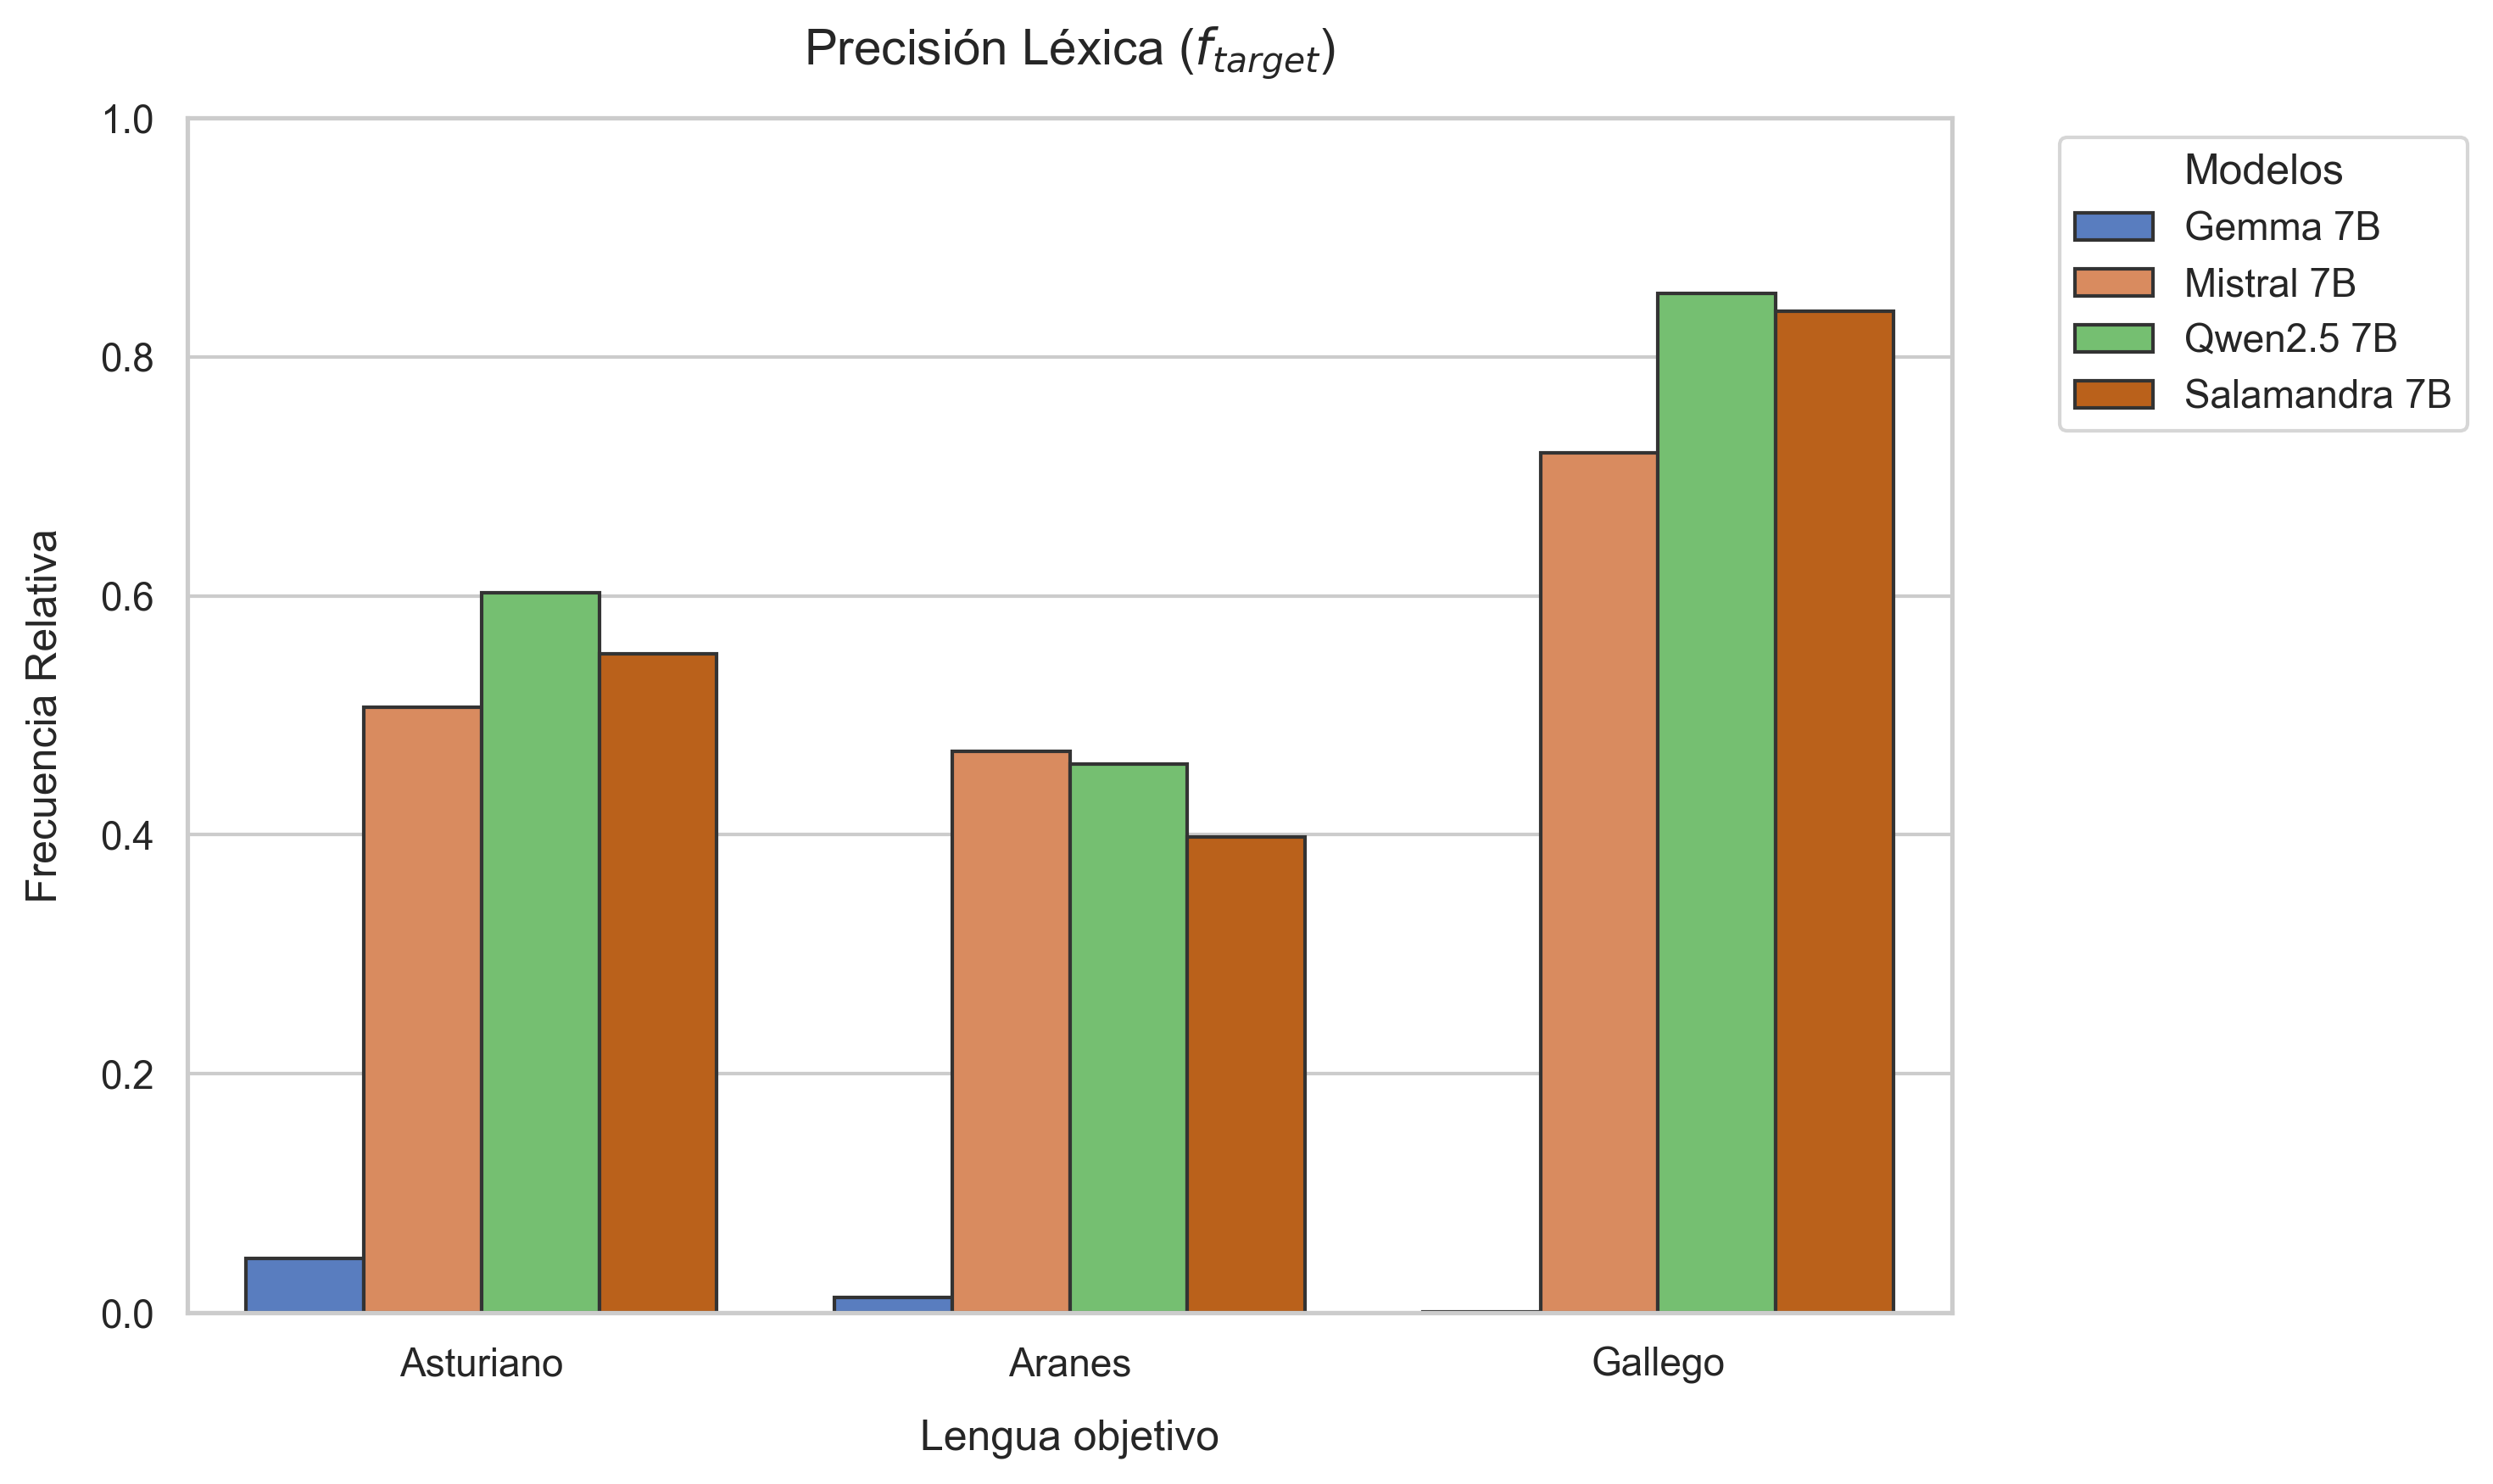
\includegraphics[width=1\textwidth]{figures/Calidad_freq_target_base.png}    
    \caption{\label{fig:resultados-base-freq-target}Freq target de los modelos por lengua. De creación propia.}
\end{figure}

\subsection{Métrica de Evaluación de las tareas}
\label{indice-agrupacion-metricas}

Con el fin de agregar el rendimiento de las tareas de evaluación en una única métrica que facilite una comparación directa y justa, se ha diseñado el siguiente índice expuesto en la Ecuación \ref{eq:indice_global}. El índice unifica las cuatro tareas de evaluación del benchmark (traducción directa, traducción de ida y vuelta, vocabulario y ortografía) mediante un promedio ponderado equiparable, donde todos los componentes están calibrados en una escala de 0 a 100:

\begin{equation}\label{eq:indice_global}
\text{\'{I}ndice Global} = \frac{chrF_{\text{trad}} + chrF_{\text{rt}} + Acc_{\text{vocab}} + Score_{\text{ort}}}{4}
\end{equation}

La traducción directa ($chrF_{\text{trad}}$) y la traducción de ida y vuelta o \textit{round-trip} ($chrF_{\text{rt}}$) introducen en la media el porcentaje de coincidencia de caracteres mediante la métrica chrF. Por su parte, la métrica de vocabulario ($Acc_{\text{vocab}}$) incorpora el porcentaje de acierto en la predicción de los términos enmascarados utilizando la métrica $\text{accuracy\_lower}$ (pasada a base 100).

El cálculo de la puntuación para la tarea de ortografía ($Score_{\text{ort}}$) se detalla en la Ecuación \ref{eq:score_ort}:

\begin{equation}\label{eq:score_ort}
\begin{split}
Score_{\text{ort}} = \max\left(-10, \min\left(100, \right.\right. & \left(\frac{\text{Err}_{\text{corregidos}}}{\text{Err}_{\text{totales}}} \times 100\right) \\ 
& - \text{Err}_{\text{nuevos}} \\ 
& \left.\left. - (\lambda \times (100 - chrF_{\text{ort}}))\right)\right)
\end{split}
\end{equation}

El puntaje se empieza calculando con el porcentaje base de éxito. Para ello, se dividen los errores corregidos por el modelo ($\text{Err}_{\text{corregidos}}$) entre los errores iniciales de la muestra ($\text{Err}_{\text{totales}}$) y se multiplica por 100. A partir de ahí, se restan dos penalizaciones:

Por un lado, los errores nuevos que introduce el modelo ($\text{Err}_{\text{nuevos}}$) se restan directamente de forma íntegra, descontando puntos por cada fallo inédito. Por otro lado, se penaliza la calidad general de la superficie textual mediante el recíproco del chrF ($100 - chrF_{\text{ort}}$), ponderado por un factor de suavizado $\lambda = 0.3$ para evitar un castigo excesivo en frases largas. Finalmente, el resultado se acota entre los 0 y los 100 puntos.

\begin{figure}[H]
    \centering
    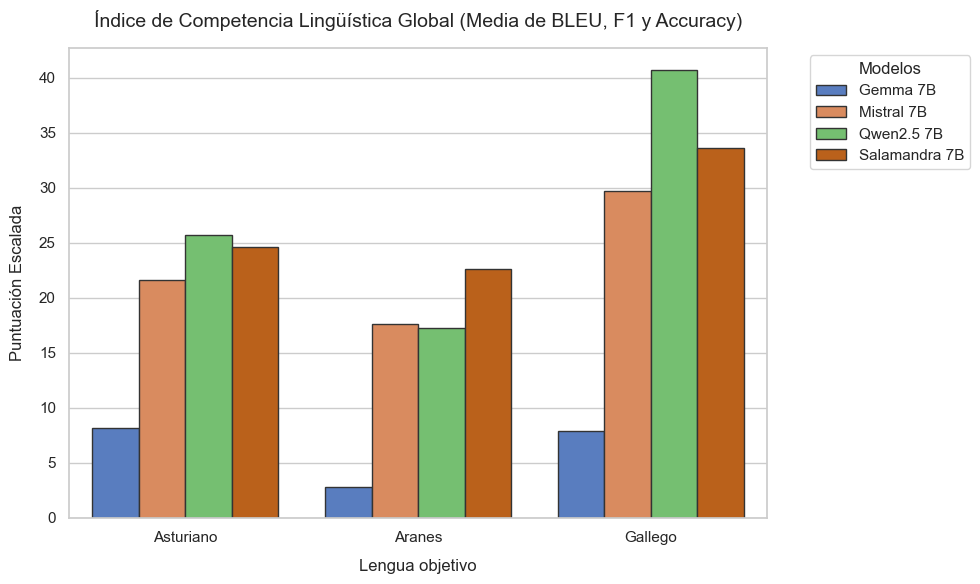
\includegraphics[width=1\textwidth]{figures/IndiceMetricas_base.png}    
    \caption{\label{fig:resultados-base-indice-metricas}Índice global de los resultados de los modelos por lengua. De creación propia.}
\end{figure}

Se puede ver en la Figura \ref{fig:resultados-base-indice-metricas} como Qwen aparte de utilizar más palabras del diccionario de las lenguas objetivo, también tiene un mejor rendimiento en el resto de tareas. La única lengua en la que pierde es en el Aranés, donde se ve que pese a ser el modelo que menos palabras usa del diccionario, aunque no por mucho, Salamandra 7B es el modelo que mejor ejecuta estas otras tareas, probablemente por su entrenamiento con gran cantidad de datos en catalán.

También se puede volver a apreciar que los modelos tienen un conocimiento bastante superior del gallego frente a otras lenguas.

A través de los ejemplos analizados en los modelos base, se ha visto que los datos de validación contienen imperfecciones puntuales, lo que puede inducir a ciertos errores en el benchmark y en el entrenamiento. No obstante, estos errores son poco comunes, garantizando una calidad suficiente para ambos procesos. Aun así, disponer de unos datos de mayor calidad proporcionaría un benchmark todavía más preciso y un entrenamiento más rico y correcto.

Con estos resultados, finalmente el modelo que se va a utilizar como base para entrenar en estas tres lenguas va a ser \textbf{Qwen 2.5 7B}.